
\documentclass[12pt]{book}

\usepackage[norsk]{babel} 
\usepackage[utf8]{inputenc}
\usepackage{graphicx}
\graphicspath{ {img/} }

\begin{document}
\clearpage

\newcommand\nbvspace[1][3]{\vspace*{\stretch{#1}}}
\newcommand\nbstretchyspace{\spaceskip0.5em plus 0.25em minus 0.25em}
\newcommand{\nbtitlestretch}{\spaceskip0.6em}
\pagestyle{empty}
\begin{center}
\bfseries
\nbvspace[1]
\Huge
{\nbtitlestretch\huge
Gubberenn Dataprogram \\}

\nbvspace[10]
\normalsize

Bruksanvisning\\
GDPKonsoll\\

\nbvspace[2]

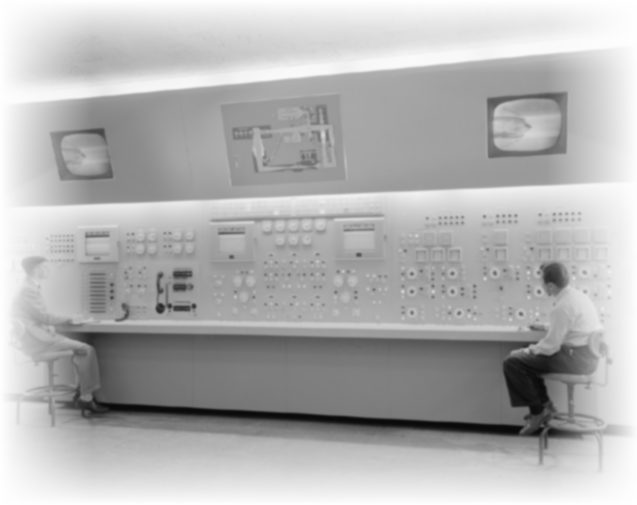
\includegraphics[width=5.0in]{gubb}
\nbvspace[15]
\normalsize

20(C)15\\
\large
Bjørkebakk og omegn Grendelag
\nbvspace[1]
\end{center}

\tableofcontents




\chapter{Bruksanvisning}

Hensikten med dette dokumentet er å forklare i detalj hvordan man kan bruke 'gubb-konsoll' -programmet på en Windows-plattform ala Windows 7 eller lignende. Programmet utfører de nødvendige beregningene i forbindelse med arrangeringen av Gubberennet. Beregningene er basert på ei input-fil som du oppretter ved hjelp av f.eks Microsoft Office Excel,  LibreOffice eller et annet egnet regnearkprogramm. 

\section{Installasjon}

Aller først må du installere programmet. Dette gjør du ved å starte programmet som heter GubbKonsollInstaller.exe

Dette vil installere noen filer på "Skrivebordet", under en katalog som heter "GubbKonsoll". Ta å åpne opp et "kommando-vidu" i Windows, og gå til denne katalogen. Når du står i 


\begin{figure}
\centering
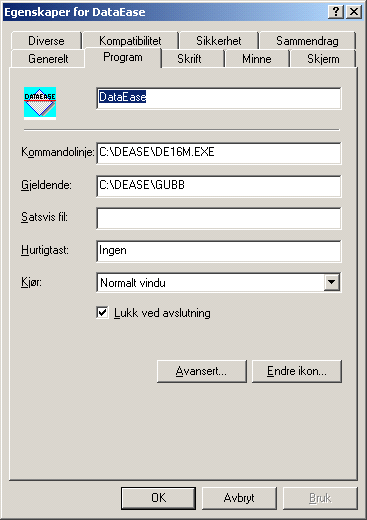
\includegraphics[width=12.0cm]{bilde}
\caption{Legg merke til  'gjeldende'}
\end{figure}


\section{Registrer brukere}

\section{Registrer anvendt tid}

\section{Registrer oppgavepoeng}

\section{Utfør beregningene}

\section{Skriv ut rapporter}


\end{document}
